\documentclass{standalone}
\usepackage{tikz}
\usetikzlibrary{arrows.meta}
\usetikzlibrary{positioning}

\begin{document}
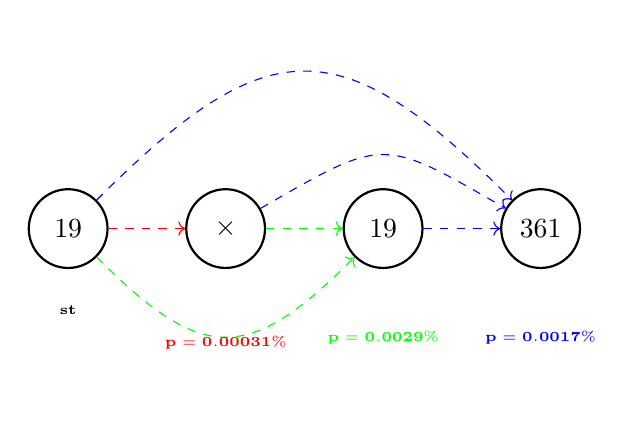
\begin{tikzpicture}[node distance=2cm, auto,
    every node/.style={circle, draw=black, thick, minimum size=1cm},
    arrow/.style={thick, -{Latex[length=3mm]}}]

  \node (w1) {19};
  \node (w2) [right of=w1] {$\times$};
  \node (w3) [right of=w2] {19};
  \node (w4) [right of=w3] {361};

  \draw[->] (w1) edge[red,dashed] (w2);
  \draw[->] (w2) edge[green,dashed] (w3);
  \draw[->] (w3) edge[blue,dashed] (w4);
  \draw[->,blue,dashed] (w1) to[out=45,in=135,looseness=1.5] (w4);
  \draw[->,blue,dashed] (w2) to[out=30,in=150,looseness=1.5] (w4);
  \draw[->,green,dashed] (w1) to[out=-45,in=-135,looseness=1.5] (w3);

  \node[draw=none,font=\tiny\ttfamily,below=0.01cm of w1] (label_w1) {$\mathbf{st}$};
  \node[draw=none,font=\tiny\ttfamily, red, below=0.01cm of w2] (label_w2) {$\mathbf{p=0.00031}\%$};
  \node[draw=none,font=\tiny\ttfamily, green, below=0.01cm of w3] (label_w3) {$\mathbf{p=0.0029}\%$};
  \node[draw=none,font=\tiny\ttfamily, blue, below=0.01cm of w4] (label_w4) {$\mathbf{p=0.0017}\%$};
\end{tikzpicture}
\end{document}
